\documentclass[twoside]{book}

% Packages required by doxygen
\usepackage{fixltx2e}
\usepackage{calc}
\usepackage{doxygen}
\usepackage[export]{adjustbox} % also loads graphicx
\usepackage{graphicx}
\usepackage[utf8]{inputenc}
\usepackage{makeidx}
\usepackage{multicol}
\usepackage{multirow}
\PassOptionsToPackage{warn}{textcomp}
\usepackage{textcomp}
\usepackage[nointegrals]{wasysym}
\usepackage[table]{xcolor}

% Font selection
\usepackage[T1]{fontenc}
\usepackage[scaled=.90]{helvet}
\usepackage{courier}
\usepackage{amssymb}
\usepackage{sectsty}
\renewcommand{\familydefault}{\sfdefault}
\allsectionsfont{%
  \fontseries{bc}\selectfont%
  \color{darkgray}%
}
\renewcommand{\DoxyLabelFont}{%
  \fontseries{bc}\selectfont%
  \color{darkgray}%
}
\newcommand{\+}{\discretionary{\mbox{\scriptsize$\hookleftarrow$}}{}{}}

% Page & text layout
\usepackage{geometry}
\geometry{%
  a4paper,%
  top=2.5cm,%
  bottom=2.5cm,%
  left=2.5cm,%
  right=2.5cm%
}
\tolerance=750
\hfuzz=15pt
\hbadness=750
\setlength{\emergencystretch}{15pt}
\setlength{\parindent}{0cm}
\setlength{\parskip}{3ex plus 2ex minus 2ex}
\makeatletter
\renewcommand{\paragraph}{%
  \@startsection{paragraph}{4}{0ex}{-1.0ex}{1.0ex}{%
    \normalfont\normalsize\bfseries\SS@parafont%
  }%
}
\renewcommand{\subparagraph}{%
  \@startsection{subparagraph}{5}{0ex}{-1.0ex}{1.0ex}{%
    \normalfont\normalsize\bfseries\SS@subparafont%
  }%
}
\makeatother

% Headers & footers
\usepackage{fancyhdr}
\pagestyle{fancyplain}
\fancyhead[LE]{\fancyplain{}{\bfseries\thepage}}
\fancyhead[CE]{\fancyplain{}{}}
\fancyhead[RE]{\fancyplain{}{\bfseries\leftmark}}
\fancyhead[LO]{\fancyplain{}{\bfseries\rightmark}}
\fancyhead[CO]{\fancyplain{}{}}
\fancyhead[RO]{\fancyplain{}{\bfseries\thepage}}
\fancyfoot[LE]{\fancyplain{}{}}
\fancyfoot[CE]{\fancyplain{}{}}
\fancyfoot[RE]{\fancyplain{}{\bfseries\scriptsize Generated by Doxygen }}
\fancyfoot[LO]{\fancyplain{}{\bfseries\scriptsize Generated by Doxygen }}
\fancyfoot[CO]{\fancyplain{}{}}
\fancyfoot[RO]{\fancyplain{}{}}
\renewcommand{\footrulewidth}{0.4pt}
\renewcommand{\chaptermark}[1]{%
  \markboth{#1}{}%
}
\renewcommand{\sectionmark}[1]{%
  \markright{\thesection\ #1}%
}

% Indices & bibliography
\usepackage{natbib}
\usepackage[titles]{tocloft}
\setcounter{tocdepth}{3}
\setcounter{secnumdepth}{5}
\makeindex

% Hyperlinks (required, but should be loaded last)
\usepackage{ifpdf}
\ifpdf
  \usepackage[pdftex,pagebackref=true]{hyperref}
\else
  \usepackage[ps2pdf,pagebackref=true]{hyperref}
\fi
\hypersetup{%
  colorlinks=true,%
  linkcolor=blue,%
  citecolor=blue,%
  unicode%
}

% Custom commands
\newcommand{\clearemptydoublepage}{%
  \newpage{\pagestyle{empty}\cleardoublepage}%
}

\usepackage{caption}
\captionsetup{labelsep=space,justification=centering,font={bf},singlelinecheck=off,skip=4pt,position=top}

%===== C O N T E N T S =====

\begin{document}

% Titlepage & ToC
\hypersetup{pageanchor=false,
             bookmarksnumbered=true,
             pdfencoding=unicode
            }
\pagenumbering{alph}
\begin{titlepage}
\vspace*{7cm}
\begin{center}%
{\Large Elevator by Jo og Siri \\[1ex]\large 1 }\\
\vspace*{1cm}
{\large Generated by Doxygen 1.8.13}\\
\end{center}
\end{titlepage}
\clearemptydoublepage
\pagenumbering{roman}
\tableofcontents
\clearemptydoublepage
\pagenumbering{arabic}
\hypersetup{pageanchor=true}

%--- Begin generated contents ---
\chapter{File Index}
\section{File List}
Here is a list of all documented files with brief descriptions\+:\begin{DoxyCompactList}
\item\contentsline{section}{source/{\bfseries channels.\+h} }{\pageref{channels_8h}}{}
\item\contentsline{section}{source/{\bfseries con\+\_\+load.\+h} }{\pageref{con__load_8h}}{}
\item\contentsline{section}{source/{\bfseries controller.\+c} }{\pageref{controller_8c}}{}
\item\contentsline{section}{source/\hyperlink{controller_8h}{controller.\+h} \\*This library contains the logic that controls the elevator movements }{\pageref{controller_8h}}{}
\item\contentsline{section}{source/{\bfseries elev.\+c} }{\pageref{elev_8c}}{}
\item\contentsline{section}{source/{\bfseries elev.\+h} }{\pageref{elev_8h}}{}
\item\contentsline{section}{source/{\bfseries elevsim.\+c} }{\pageref{elevsim_8c}}{}
\item\contentsline{section}{source/{\bfseries elevsim.\+h} }{\pageref{elevsim_8h}}{}
\item\contentsline{section}{source/{\bfseries io.\+c} }{\pageref{io_8c}}{}
\item\contentsline{section}{source/{\bfseries io.\+h} }{\pageref{io_8h}}{}
\item\contentsline{section}{source/{\bfseries main.\+c} }{\pageref{main_8c}}{}
\item\contentsline{section}{source/{\bfseries state\+\_\+machine.\+c} }{\pageref{state__machine_8c}}{}
\item\contentsline{section}{source/\hyperlink{state__machine_8h}{state\+\_\+machine.\+h} \\*This module contains the state machine ant the initialize function }{\pageref{state__machine_8h}}{}
\item\contentsline{section}{source/{\bfseries timer.\+c} }{\pageref{timer_8c}}{}
\item\contentsline{section}{source/\hyperlink{timer_8h}{timer.\+h} \\*A simple module to controll the timer of the door }{\pageref{timer_8h}}{}
\end{DoxyCompactList}

\chapter{File Documentation}
\hypertarget{controller_8h}{}\section{source/controller.h File Reference}
\label{controller_8h}\index{source/controller.\+h@{source/controller.\+h}}


This library contains the logic that controls the elevator movements.  


{\ttfamily \#include \char`\"{}elev.\+h\char`\"{}}\\*
Include dependency graph for controller.\+h\+:
\nopagebreak
\begin{figure}[H]
\begin{center}
\leavevmode
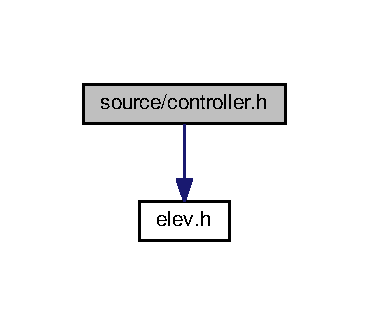
\includegraphics[width=177pt]{controller_8h__incl}
\end{center}
\end{figure}
This graph shows which files directly or indirectly include this file\+:
\nopagebreak
\begin{figure}[H]
\begin{center}
\leavevmode
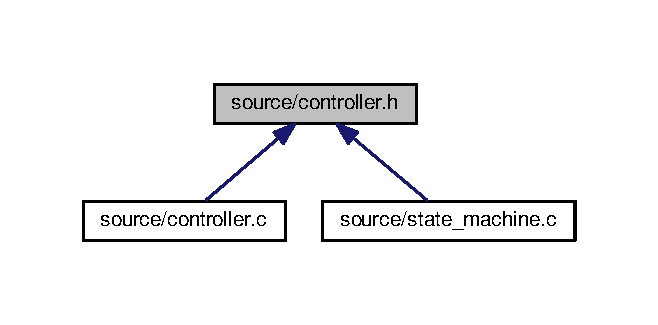
\includegraphics[width=316pt]{controller_8h__dep__incl}
\end{center}
\end{figure}
\subsection*{Typedefs}
\begin{DoxyCompactItemize}
\item 
typedef enum \hyperlink{controller_8h_aa19be6305a5a4485e1e70de70ed7d677}{states} \hyperlink{controller_8h_afe776354e225815b2fdb1308becfa9d0}{states\+\_\+t}
\end{DoxyCompactItemize}
\subsection*{Enumerations}
\begin{DoxyCompactItemize}
\item 
enum \hyperlink{controller_8h_aa19be6305a5a4485e1e70de70ed7d677}{states} \{ \hyperlink{controller_8h_aa19be6305a5a4485e1e70de70ed7d677a0cb1b2c6a7db1f1084886c98909a3f36}{I\+N\+IT} = 0, 
\hyperlink{controller_8h_aa19be6305a5a4485e1e70de70ed7d677afd6a0e4343048b10646dd2976cc5ad18}{I\+D\+LE}, 
\hyperlink{controller_8h_aa19be6305a5a4485e1e70de70ed7d677a1061be6c3fb88d32829cba6f6b2be304}{R\+U\+N\+N\+I\+NG}, 
\hyperlink{controller_8h_aa19be6305a5a4485e1e70de70ed7d677a11915658ade106027bd75056b907539d}{D\+O\+O\+R\+\_\+\+O\+P\+EN}
 \}
\end{DoxyCompactItemize}
\subsection*{Functions}
\begin{DoxyCompactItemize}
\item 
int \hyperlink{controller_8h_af29666bc4492206c0a8f18025da5fb0a}{controller\+\_\+delete\+\_\+order\+\_\+at\+\_\+floor} (int floor)
\begin{DoxyCompactList}\small\item\em Deletes all orders at a floor. \end{DoxyCompactList}\item 
int \hyperlink{controller_8h_a6acb7bf61ebd1aadc637485d54bba761}{controller\+\_\+delete\+\_\+all\+\_\+orders} ()
\begin{DoxyCompactList}\small\item\em Deletes all orders at all floors. \end{DoxyCompactList}\item 
int \hyperlink{controller_8h_a0908010f57221cdf378321156defbf13}{controller\+\_\+update\+\_\+orders} ()
\begin{DoxyCompactList}\small\item\em Checking buttons\+: C\+O\+M\+M\+A\+ND, UP and D\+O\+WN and updates the ordes array. \end{DoxyCompactList}\item 
int \hyperlink{controller_8h_a0b9e23bbfadec5ee839e8e9157d26081}{controller\+\_\+update\+\_\+elev\+\_\+postition} (int $\ast$p\+\_\+current\+\_\+floor)
\begin{DoxyCompactList}\small\item\em Chekcs if the elevator has reached a floor and updates the current floor acordingly. \end{DoxyCompactList}\item 
int \hyperlink{controller_8h_ab0c894bcc724527bbdd69b2ee25f871b}{controller\+\_\+order\+\_\+at\+\_\+floor} (elev\+\_\+motor\+\_\+direction\+\_\+t $\ast$p\+\_\+priority\+\_\+dir, elev\+\_\+motor\+\_\+direction\+\_\+t elev\+\_\+dir)
\begin{DoxyCompactList}\small\item\em Checking if there are orders at current floor and if the eleveator should stop. It also checks if the elevator is about to move bellow the bootom floor or above the top floor. \end{DoxyCompactList}\item 
int \hyperlink{controller_8h_a2f2f6e3d67a596407276d09193936bd2}{controller\+\_\+order\+\_\+at\+\_\+current\+\_\+floor} (elev\+\_\+motor\+\_\+direction\+\_\+t $\ast$p\+\_\+elev\+\_\+dir, int e\+\_\+stopped, int current\+\_\+floor, int $\ast$p\+\_\+dir\+\_\+switch)
\begin{DoxyCompactList}\small\item\em Used to check if the order is at the current floor so the elev can open the doors. It is also used to check if the elevator is actually at the floor it thinks it is after an emergency stop and if the elevator switched direction to get back to the floor it thinks it is at. \end{DoxyCompactList}\item 
int \hyperlink{controller_8h_a8b5c053572a9fa9284474b13fc6ca666}{controller\+\_\+orders\+\_\+bellow} (elev\+\_\+motor\+\_\+direction\+\_\+t $\ast$p\+\_\+priority\+\_\+dir, int current\+\_\+floor)
\begin{DoxyCompactList}\small\item\em Checks if there are any orders of interest above current floor. \end{DoxyCompactList}\item 
int \hyperlink{controller_8h_aea909d8a658a7fd1c2e519a3ae13fe5c}{controller\+\_\+orders\+\_\+above} (elev\+\_\+motor\+\_\+direction\+\_\+t $\ast$p\+\_\+priority\+\_\+dir, int current\+\_\+floor)
\begin{DoxyCompactList}\small\item\em Checks if there are any orders of interest above current floor. \end{DoxyCompactList}\item 
int \hyperlink{controller_8h_a0590c6fc85919f2e6c92facae7d2d97d}{controller\+\_\+e\+\_\+stop} (int $\ast$p\+\_\+e\+\_\+stopped, elev\+\_\+motor\+\_\+direction\+\_\+t $\ast$p\+\_\+elev\+\_\+dir, elev\+\_\+motor\+\_\+direction\+\_\+t $\ast$p\+\_\+priority\+\_\+dir, \hyperlink{controller_8h_afe776354e225815b2fdb1308becfa9d0}{states\+\_\+t} $\ast$p\+\_\+elev\+\_\+state)
\begin{DoxyCompactList}\small\item\em Checking emergency stop and if an emergency stop has occured it deside if it\textquotesingle{}s going to open the door or just stand still. \end{DoxyCompactList}\item 
int \hyperlink{controller_8h_a2d90abbd2fa39d3ea75f0802eb3529d9}{controller\+\_\+update\+\_\+lamps} ()
\begin{DoxyCompactList}\small\item\em Controll the lamps of whitch floor the elevator is or last was located in, floorpanel and elevatorepanel, but not the emergency lamp. \end{DoxyCompactList}\end{DoxyCompactItemize}


\subsection{Detailed Description}
This library contains the logic that controls the elevator movements. 



\subsection{Typedef Documentation}
\index{controller.\+h@{controller.\+h}!states\+\_\+t@{states\+\_\+t}}
\index{states\+\_\+t@{states\+\_\+t}!controller.\+h@{controller.\+h}}
\subsubsection[{\texorpdfstring{states\+\_\+t}{states_t}}]{\setlength{\rightskip}{0pt plus 5cm}typedef enum {\bf states}  {\bf states\+\_\+t}}\hypertarget{controller_8h_afe776354e225815b2fdb1308becfa9d0}{}\label{controller_8h_afe776354e225815b2fdb1308becfa9d0}
Contains the state the elevator possible can be located in 

\subsection{Enumeration Type Documentation}
\index{controller.\+h@{controller.\+h}!states@{states}}
\index{states@{states}!controller.\+h@{controller.\+h}}
\subsubsection[{\texorpdfstring{states}{states}}]{\setlength{\rightskip}{0pt plus 5cm}enum {\bf states}}\hypertarget{controller_8h_aa19be6305a5a4485e1e70de70ed7d677}{}\label{controller_8h_aa19be6305a5a4485e1e70de70ed7d677}
Contains the state the elevator possible can be located in \begin{Desc}
\item[Enumerator]\par
\begin{description}
\index{I\+N\+IT@{I\+N\+IT}!controller.\+h@{controller.\+h}}\index{controller.\+h@{controller.\+h}!I\+N\+IT@{I\+N\+IT}}\item[{\em 
I\+N\+IT\hypertarget{controller_8h_aa19be6305a5a4485e1e70de70ed7d677a0cb1b2c6a7db1f1084886c98909a3f36}{}\label{controller_8h_aa19be6305a5a4485e1e70de70ed7d677a0cb1b2c6a7db1f1084886c98909a3f36}
}]initialing elevator and state machine \index{I\+D\+LE@{I\+D\+LE}!controller.\+h@{controller.\+h}}\index{controller.\+h@{controller.\+h}!I\+D\+LE@{I\+D\+LE}}\item[{\em 
I\+D\+LE\hypertarget{controller_8h_aa19be6305a5a4485e1e70de70ed7d677afd6a0e4343048b10646dd2976cc5ad18}{}\label{controller_8h_aa19be6305a5a4485e1e70de70ed7d677afd6a0e4343048b10646dd2976cc5ad18}
}]wating for orders \index{R\+U\+N\+N\+I\+NG@{R\+U\+N\+N\+I\+NG}!controller.\+h@{controller.\+h}}\index{controller.\+h@{controller.\+h}!R\+U\+N\+N\+I\+NG@{R\+U\+N\+N\+I\+NG}}\item[{\em 
R\+U\+N\+N\+I\+NG\hypertarget{controller_8h_aa19be6305a5a4485e1e70de70ed7d677a1061be6c3fb88d32829cba6f6b2be304}{}\label{controller_8h_aa19be6305a5a4485e1e70de70ed7d677a1061be6c3fb88d32829cba6f6b2be304}
}]running the elevator \index{D\+O\+O\+R\+\_\+\+O\+P\+EN@{D\+O\+O\+R\+\_\+\+O\+P\+EN}!controller.\+h@{controller.\+h}}\index{controller.\+h@{controller.\+h}!D\+O\+O\+R\+\_\+\+O\+P\+EN@{D\+O\+O\+R\+\_\+\+O\+P\+EN}}\item[{\em 
D\+O\+O\+R\+\_\+\+O\+P\+EN\hypertarget{controller_8h_aa19be6305a5a4485e1e70de70ed7d677a11915658ade106027bd75056b907539d}{}\label{controller_8h_aa19be6305a5a4485e1e70de70ed7d677a11915658ade106027bd75056b907539d}
}]the door is open \end{description}
\end{Desc}


Definition at line 13 of file controller.\+h.



\subsection{Function Documentation}
\index{controller.\+h@{controller.\+h}!controller\+\_\+delete\+\_\+all\+\_\+orders@{controller\+\_\+delete\+\_\+all\+\_\+orders}}
\index{controller\+\_\+delete\+\_\+all\+\_\+orders@{controller\+\_\+delete\+\_\+all\+\_\+orders}!controller.\+h@{controller.\+h}}
\subsubsection[{\texorpdfstring{controller\+\_\+delete\+\_\+all\+\_\+orders()}{controller_delete_all_orders()}}]{\setlength{\rightskip}{0pt plus 5cm}int controller\+\_\+delete\+\_\+all\+\_\+orders (
\begin{DoxyParamCaption}
{}
\end{DoxyParamCaption}
)}\hypertarget{controller_8h_a6acb7bf61ebd1aadc637485d54bba761}{}\label{controller_8h_a6acb7bf61ebd1aadc637485d54bba761}


Deletes all orders at all floors. 

\begin{DoxyReturn}{Returns}
0 when done. 
\end{DoxyReturn}


Definition at line 24 of file controller.\+c.

\index{controller.\+h@{controller.\+h}!controller\+\_\+delete\+\_\+order\+\_\+at\+\_\+floor@{controller\+\_\+delete\+\_\+order\+\_\+at\+\_\+floor}}
\index{controller\+\_\+delete\+\_\+order\+\_\+at\+\_\+floor@{controller\+\_\+delete\+\_\+order\+\_\+at\+\_\+floor}!controller.\+h@{controller.\+h}}
\subsubsection[{\texorpdfstring{controller\+\_\+delete\+\_\+order\+\_\+at\+\_\+floor(int floor)}{controller_delete_order_at_floor(int floor)}}]{\setlength{\rightskip}{0pt plus 5cm}int controller\+\_\+delete\+\_\+order\+\_\+at\+\_\+floor (
\begin{DoxyParamCaption}
\item[{int}]{floor}
\end{DoxyParamCaption}
)}\hypertarget{controller_8h_af29666bc4492206c0a8f18025da5fb0a}{}\label{controller_8h_af29666bc4492206c0a8f18025da5fb0a}


Deletes all orders at a floor. 


\begin{DoxyParams}[1]{Parameters}
\mbox{\tt in}  & {\em floor} & Where orderes wil be destructed.\\
\hline
\end{DoxyParams}
\begin{DoxyReturn}{Returns}
0 when done 
\end{DoxyReturn}


Definition at line 17 of file controller.\+c.

\index{controller.\+h@{controller.\+h}!controller\+\_\+e\+\_\+stop@{controller\+\_\+e\+\_\+stop}}
\index{controller\+\_\+e\+\_\+stop@{controller\+\_\+e\+\_\+stop}!controller.\+h@{controller.\+h}}
\subsubsection[{\texorpdfstring{controller\+\_\+e\+\_\+stop(int $\ast$p\+\_\+e\+\_\+stopped, elev\+\_\+motor\+\_\+direction\+\_\+t $\ast$p\+\_\+elev\+\_\+dir, elev\+\_\+motor\+\_\+direction\+\_\+t $\ast$p\+\_\+priority\+\_\+dir, states\+\_\+t $\ast$p\+\_\+elev\+\_\+state)}{controller_e_stop(int *p_e_stopped, elev_motor_direction_t *p_elev_dir, elev_motor_direction_t *p_priority_dir, states_t *p_elev_state)}}]{\setlength{\rightskip}{0pt plus 5cm}int controller\+\_\+e\+\_\+stop (
\begin{DoxyParamCaption}
\item[{int $\ast$}]{p\+\_\+e\+\_\+stopped, }
\item[{elev\+\_\+motor\+\_\+direction\+\_\+t $\ast$}]{p\+\_\+elev\+\_\+dir, }
\item[{elev\+\_\+motor\+\_\+direction\+\_\+t $\ast$}]{p\+\_\+priority\+\_\+dir, }
\item[{{\bf states\+\_\+t} $\ast$}]{p\+\_\+elev\+\_\+state}
\end{DoxyParamCaption}
)}\hypertarget{controller_8h_a0590c6fc85919f2e6c92facae7d2d97d}{}\label{controller_8h_a0590c6fc85919f2e6c92facae7d2d97d}


Checking emergency stop and if an emergency stop has occured it deside if it\textquotesingle{}s going to open the door or just stand still. 


\begin{DoxyParams}[1]{Parameters}
\mbox{\tt in,out}  & {\em e\+\_\+stopped} & Takes in a 0 or not 0 integer to tell if an emergiency stop has occured. \\
\hline
\mbox{\tt in}  & {\em elev\+\_\+dir} & The elevation direction of movement. \\
\hline
\mbox{\tt in,out}  & {\em priority\+\_\+dir} & Orders in this direction are prioritized. \\
\hline
\mbox{\tt in,out}  & {\em elev\+\_\+state} & The state the elevator currently is given from the state machine.\\
\hline
\end{DoxyParams}
\begin{DoxyReturn}{Returns}
0 if the fuction does not take in a active emergency signal and therefore do nothing, 1 if it gets a stopsignal. 
\end{DoxyReturn}


Definition at line 194 of file controller.\+c.

\index{controller.\+h@{controller.\+h}!controller\+\_\+order\+\_\+at\+\_\+current\+\_\+floor@{controller\+\_\+order\+\_\+at\+\_\+current\+\_\+floor}}
\index{controller\+\_\+order\+\_\+at\+\_\+current\+\_\+floor@{controller\+\_\+order\+\_\+at\+\_\+current\+\_\+floor}!controller.\+h@{controller.\+h}}
\subsubsection[{\texorpdfstring{controller\+\_\+order\+\_\+at\+\_\+current\+\_\+floor(elev\+\_\+motor\+\_\+direction\+\_\+t $\ast$p\+\_\+elev\+\_\+dir, int e\+\_\+stopped, int current\+\_\+floor, int $\ast$p\+\_\+dir\+\_\+switch)}{controller_order_at_current_floor(elev_motor_direction_t *p_elev_dir, int e_stopped, int current_floor, int *p_dir_switch)}}]{\setlength{\rightskip}{0pt plus 5cm}int controller\+\_\+order\+\_\+at\+\_\+current\+\_\+floor (
\begin{DoxyParamCaption}
\item[{elev\+\_\+motor\+\_\+direction\+\_\+t $\ast$}]{p\+\_\+elev\+\_\+dir, }
\item[{int}]{e\+\_\+stopped, }
\item[{int}]{current\+\_\+floor, }
\item[{int $\ast$}]{p\+\_\+dir\+\_\+switch}
\end{DoxyParamCaption}
)}\hypertarget{controller_8h_a2f2f6e3d67a596407276d09193936bd2}{}\label{controller_8h_a2f2f6e3d67a596407276d09193936bd2}


Used to check if the order is at the current floor so the elev can open the doors. It is also used to check if the elevator is actually at the floor it thinks it is after an emergency stop and if the elevator switched direction to get back to the floor it thinks it is at. 


\begin{DoxyParams}[1]{Parameters}
\mbox{\tt in,out}  & {\em p\+\_\+elev\+\_\+dir} & The elevators direction of movement. \\
\hline
\mbox{\tt in}  & {\em e\+\_\+stopped} & 0 or not 0 integer to tell if an emergency stop has occured. \\
\hline
\mbox{\tt in}  & {\em current\+\_\+floor} & The floor which the elevator last moved by. \\
\hline
\mbox{\tt in,out}  & {\em p\+\_\+dir\+\_\+switch} & A variable to tell if the elevator has switched direction after an emergency stop occured.\\
\hline
\end{DoxyParams}
\begin{DoxyReturn}{Returns}
1 when there exists an order in the current floor, 2 if it\textquotesingle{}s been an emergency stop and it\textquotesingle{}s supposed to switch direction or 0 if not 1 or 2. 
\end{DoxyReturn}
\begin{DoxyWarning}{Warning}
When called this function may change {\ttfamily p\+\_\+dir\+\_\+switch} and therfore the next call will give a diffrent result. 
\end{DoxyWarning}


Definition at line 99 of file controller.\+c.

\index{controller.\+h@{controller.\+h}!controller\+\_\+order\+\_\+at\+\_\+floor@{controller\+\_\+order\+\_\+at\+\_\+floor}}
\index{controller\+\_\+order\+\_\+at\+\_\+floor@{controller\+\_\+order\+\_\+at\+\_\+floor}!controller.\+h@{controller.\+h}}
\subsubsection[{\texorpdfstring{controller\+\_\+order\+\_\+at\+\_\+floor(elev\+\_\+motor\+\_\+direction\+\_\+t $\ast$p\+\_\+priority\+\_\+dir, elev\+\_\+motor\+\_\+direction\+\_\+t elev\+\_\+dir)}{controller_order_at_floor(elev_motor_direction_t *p_priority_dir, elev_motor_direction_t elev_dir)}}]{\setlength{\rightskip}{0pt plus 5cm}int controller\+\_\+order\+\_\+at\+\_\+floor (
\begin{DoxyParamCaption}
\item[{elev\+\_\+motor\+\_\+direction\+\_\+t $\ast$}]{p\+\_\+priority\+\_\+dir, }
\item[{elev\+\_\+motor\+\_\+direction\+\_\+t}]{elev\+\_\+dir}
\end{DoxyParamCaption}
)}\hypertarget{controller_8h_ab0c894bcc724527bbdd69b2ee25f871b}{}\label{controller_8h_ab0c894bcc724527bbdd69b2ee25f871b}


Checking if there are orders at current floor and if the eleveator should stop. It also checks if the elevator is about to move bellow the bootom floor or above the top floor. 


\begin{DoxyParams}[1]{Parameters}
\mbox{\tt in}  & {\em p\+\_\+priority\+\_\+dir} & Orders in this direction is prioritized. \\
\hline
\mbox{\tt in}  & {\em elev\+\_\+dir} & The elevators direction of movement.\\
\hline
\end{DoxyParams}
\begin{DoxyReturn}{Returns}
0 when done. 
\end{DoxyReturn}


Definition at line 66 of file controller.\+c.

\index{controller.\+h@{controller.\+h}!controller\+\_\+orders\+\_\+above@{controller\+\_\+orders\+\_\+above}}
\index{controller\+\_\+orders\+\_\+above@{controller\+\_\+orders\+\_\+above}!controller.\+h@{controller.\+h}}
\subsubsection[{\texorpdfstring{controller\+\_\+orders\+\_\+above(elev\+\_\+motor\+\_\+direction\+\_\+t $\ast$p\+\_\+priority\+\_\+dir, int current\+\_\+floor)}{controller_orders_above(elev_motor_direction_t *p_priority_dir, int current_floor)}}]{\setlength{\rightskip}{0pt plus 5cm}int controller\+\_\+orders\+\_\+above (
\begin{DoxyParamCaption}
\item[{elev\+\_\+motor\+\_\+direction\+\_\+t $\ast$}]{p\+\_\+priority\+\_\+dir, }
\item[{int}]{current\+\_\+floor}
\end{DoxyParamCaption}
)}\hypertarget{controller_8h_aea909d8a658a7fd1c2e519a3ae13fe5c}{}\label{controller_8h_aea909d8a658a7fd1c2e519a3ae13fe5c}


Checks if there are any orders of interest above current floor. 


\begin{DoxyParams}[1]{Parameters}
\mbox{\tt in,out}  & {\em p\+\_\+priority\+\_\+dir} & Orders in this direction is prioritized. If this equals D\+I\+R\+N\+\_\+\+S\+T\+OP this function may change it. \\
\hline
\mbox{\tt in}  & {\em current\+\_\+floor} & The floor which the elevator last moved by.\\
\hline
\end{DoxyParams}
\begin{DoxyReturn}{Returns}
1 if order of interest above, 0 if not. 
\end{DoxyReturn}


Definition at line 163 of file controller.\+c.

\index{controller.\+h@{controller.\+h}!controller\+\_\+orders\+\_\+bellow@{controller\+\_\+orders\+\_\+bellow}}
\index{controller\+\_\+orders\+\_\+bellow@{controller\+\_\+orders\+\_\+bellow}!controller.\+h@{controller.\+h}}
\subsubsection[{\texorpdfstring{controller\+\_\+orders\+\_\+bellow(elev\+\_\+motor\+\_\+direction\+\_\+t $\ast$p\+\_\+priority\+\_\+dir, int current\+\_\+floor)}{controller_orders_bellow(elev_motor_direction_t *p_priority_dir, int current_floor)}}]{\setlength{\rightskip}{0pt plus 5cm}int controller\+\_\+orders\+\_\+bellow (
\begin{DoxyParamCaption}
\item[{elev\+\_\+motor\+\_\+direction\+\_\+t $\ast$}]{p\+\_\+priority\+\_\+dir, }
\item[{int}]{current\+\_\+floor}
\end{DoxyParamCaption}
)}\hypertarget{controller_8h_a8b5c053572a9fa9284474b13fc6ca666}{}\label{controller_8h_a8b5c053572a9fa9284474b13fc6ca666}


Checks if there are any orders of interest above current floor. 


\begin{DoxyParams}[1]{Parameters}
\mbox{\tt in,out}  & {\em p\+\_\+priority\+\_\+dir} & Orders in this direction is prioritized. If this equals D\+I\+R\+N\+\_\+\+S\+T\+OP this function may change it. \\
\hline
\mbox{\tt in}  & {\em current\+\_\+floor} & The floor which the elevator last moved by.\\
\hline
\end{DoxyParams}
\begin{DoxyReturn}{Returns}
1 if order of interest bellow, 0 if not. 
\end{DoxyReturn}


Definition at line 132 of file controller.\+c.

\index{controller.\+h@{controller.\+h}!controller\+\_\+update\+\_\+elev\+\_\+postition@{controller\+\_\+update\+\_\+elev\+\_\+postition}}
\index{controller\+\_\+update\+\_\+elev\+\_\+postition@{controller\+\_\+update\+\_\+elev\+\_\+postition}!controller.\+h@{controller.\+h}}
\subsubsection[{\texorpdfstring{controller\+\_\+update\+\_\+elev\+\_\+postition(int $\ast$p\+\_\+current\+\_\+floor)}{controller_update_elev_postition(int *p_current_floor)}}]{\setlength{\rightskip}{0pt plus 5cm}int controller\+\_\+update\+\_\+elev\+\_\+postition (
\begin{DoxyParamCaption}
\item[{int $\ast$}]{p\+\_\+current\+\_\+floor}
\end{DoxyParamCaption}
)}\hypertarget{controller_8h_a0b9e23bbfadec5ee839e8e9157d26081}{}\label{controller_8h_a0b9e23bbfadec5ee839e8e9157d26081}


Chekcs if the elevator has reached a floor and updates the current floor acordingly. 


\begin{DoxyParams}{Parameters}
{\em p\+\_\+current\+\_\+floor} & A variable that contains the floor number.\\
\hline
\end{DoxyParams}
\begin{DoxyReturn}{Returns}
0 when done. 
\end{DoxyReturn}


Definition at line 54 of file controller.\+c.

\index{controller.\+h@{controller.\+h}!controller\+\_\+update\+\_\+lamps@{controller\+\_\+update\+\_\+lamps}}
\index{controller\+\_\+update\+\_\+lamps@{controller\+\_\+update\+\_\+lamps}!controller.\+h@{controller.\+h}}
\subsubsection[{\texorpdfstring{controller\+\_\+update\+\_\+lamps()}{controller_update_lamps()}}]{\setlength{\rightskip}{0pt plus 5cm}int controller\+\_\+update\+\_\+lamps (
\begin{DoxyParamCaption}
{}
\end{DoxyParamCaption}
)}\hypertarget{controller_8h_a2d90abbd2fa39d3ea75f0802eb3529d9}{}\label{controller_8h_a2d90abbd2fa39d3ea75f0802eb3529d9}


Controll the lamps of whitch floor the elevator is or last was located in, floorpanel and elevatorepanel, but not the emergency lamp. 

\begin{DoxyReturn}{Returns}
0 when the function do it\textquotesingle{}s job and succeed. 
\end{DoxyReturn}


Definition at line 221 of file controller.\+c.

\index{controller.\+h@{controller.\+h}!controller\+\_\+update\+\_\+orders@{controller\+\_\+update\+\_\+orders}}
\index{controller\+\_\+update\+\_\+orders@{controller\+\_\+update\+\_\+orders}!controller.\+h@{controller.\+h}}
\subsubsection[{\texorpdfstring{controller\+\_\+update\+\_\+orders()}{controller_update_orders()}}]{\setlength{\rightskip}{0pt plus 5cm}int controller\+\_\+update\+\_\+orders (
\begin{DoxyParamCaption}
{}
\end{DoxyParamCaption}
)}\hypertarget{controller_8h_a0908010f57221cdf378321156defbf13}{}\label{controller_8h_a0908010f57221cdf378321156defbf13}


Checking buttons\+: C\+O\+M\+M\+A\+ND, UP and D\+O\+WN and updates the ordes array. 

\begin{DoxyReturn}{Returns}
0 when done. 
\end{DoxyReturn}


Definition at line 31 of file controller.\+c.


\hypertarget{state__machine_8h}{}\section{source/state\+\_\+machine.h File Reference}
\label{state__machine_8h}\index{source/state\+\_\+machine.\+h@{source/state\+\_\+machine.\+h}}


This module contains the state machine ant the initialize function.  


{\ttfamily \#include $<$stdio.\+h$>$}\\*
Include dependency graph for state\+\_\+machine.\+h\+:
\nopagebreak
\begin{figure}[H]
\begin{center}
\leavevmode
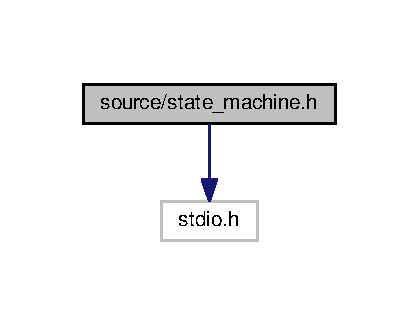
\includegraphics[width=201pt]{state__machine_8h__incl}
\end{center}
\end{figure}
This graph shows which files directly or indirectly include this file\+:
\nopagebreak
\begin{figure}[H]
\begin{center}
\leavevmode
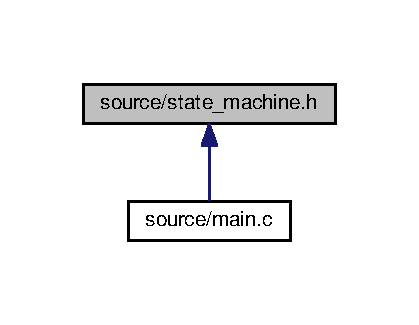
\includegraphics[width=201pt]{state__machine_8h__dep__incl}
\end{center}
\end{figure}
\subsection*{Functions}
\begin{DoxyCompactItemize}
\item 
int \hyperlink{state__machine_8h_adf22476b091b134f6bc786c066944441}{state\+\_\+machine\+\_\+init} ()
\begin{DoxyCompactList}\small\item\em Initializes the elevator by placing it at a known floor. \end{DoxyCompactList}\item 
int \hyperlink{state__machine_8h_ad2dedf94c6d80fdbebcf166241a0ed61}{state\+\_\+machine\+\_\+run} ()
\begin{DoxyCompactList}\small\item\em This is the state machine. Just run it from main and watch the magic. \end{DoxyCompactList}\end{DoxyCompactItemize}


\subsection{Detailed Description}
This module contains the state machine ant the initialize function. 



\subsection{Function Documentation}
\index{state\+\_\+machine.\+h@{state\+\_\+machine.\+h}!state\+\_\+machine\+\_\+init@{state\+\_\+machine\+\_\+init}}
\index{state\+\_\+machine\+\_\+init@{state\+\_\+machine\+\_\+init}!state\+\_\+machine.\+h@{state\+\_\+machine.\+h}}
\subsubsection[{\texorpdfstring{state\+\_\+machine\+\_\+init()}{state_machine_init()}}]{\setlength{\rightskip}{0pt plus 5cm}int state\+\_\+machine\+\_\+init (
\begin{DoxyParamCaption}
{}
\end{DoxyParamCaption}
)}\hypertarget{state__machine_8h_adf22476b091b134f6bc786c066944441}{}\label{state__machine_8h_adf22476b091b134f6bc786c066944441}


Initializes the elevator by placing it at a known floor. 

\begin{DoxyReturn}{Returns}
0 when done. 
\end{DoxyReturn}


Definition at line 5 of file state\+\_\+machine.\+c.

\index{state\+\_\+machine.\+h@{state\+\_\+machine.\+h}!state\+\_\+machine\+\_\+run@{state\+\_\+machine\+\_\+run}}
\index{state\+\_\+machine\+\_\+run@{state\+\_\+machine\+\_\+run}!state\+\_\+machine.\+h@{state\+\_\+machine.\+h}}
\subsubsection[{\texorpdfstring{state\+\_\+machine\+\_\+run()}{state_machine_run()}}]{\setlength{\rightskip}{0pt plus 5cm}int state\+\_\+machine\+\_\+run (
\begin{DoxyParamCaption}
{}
\end{DoxyParamCaption}
)}\hypertarget{state__machine_8h_ad2dedf94c6d80fdbebcf166241a0ed61}{}\label{state__machine_8h_ad2dedf94c6d80fdbebcf166241a0ed61}


This is the state machine. Just run it from main and watch the magic. 

\begin{DoxyReturn}{Returns}
0 when done. 
\end{DoxyReturn}


Definition at line 23 of file state\+\_\+machine.\+c.


\hypertarget{timer_8h}{}\section{source/timer.h File Reference}
\label{timer_8h}\index{source/timer.\+h@{source/timer.\+h}}


A simple module to controll the timer of the door.  


{\ttfamily \#include $<$stdio.\+h$>$}\newline
{\ttfamily \#include $<$time.\+h$>$}\newline
Include dependency graph for timer.\+h\+:
\nopagebreak
\begin{figure}[H]
\begin{center}
\leavevmode
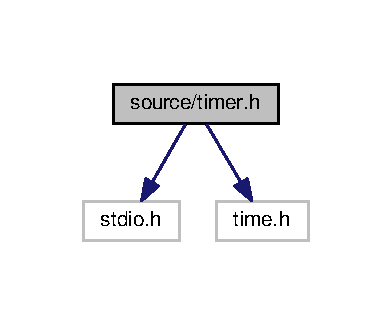
\includegraphics[width=188pt]{timer_8h__incl}
\end{center}
\end{figure}
This graph shows which files directly or indirectly include this file\+:
\nopagebreak
\begin{figure}[H]
\begin{center}
\leavevmode
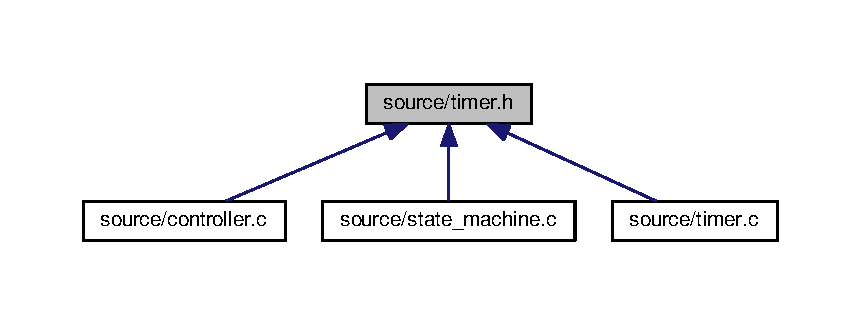
\includegraphics[width=350pt]{timer_8h__dep__incl}
\end{center}
\end{figure}
\subsection*{Functions}
\begin{DoxyCompactItemize}
\item 
\mbox{\Hypertarget{timer_8h_a38de4e764d5a9817f0886463eb462330}\label{timer_8h_a38de4e764d5a9817f0886463eb462330}} 
void \hyperlink{timer_8h_a38de4e764d5a9817f0886463eb462330}{timer\+\_\+start\+\_\+timer} (void)
\begin{DoxyCompactList}\small\item\em Sets the starttime to the current time. \end{DoxyCompactList}\item 
int \hyperlink{timer_8h_acecc2c1f586347f7ce2c8fa1cc048f7e}{timer\+\_\+time\+\_\+out} (void)
\begin{DoxyCompactList}\small\item\em Checks if it\textquotesingle{}s three seconds since the starttime. \end{DoxyCompactList}\end{DoxyCompactItemize}


\subsection{Detailed Description}
A simple module to controll the timer of the door. 



\subsection{Function Documentation}
\mbox{\Hypertarget{timer_8h_acecc2c1f586347f7ce2c8fa1cc048f7e}\label{timer_8h_acecc2c1f586347f7ce2c8fa1cc048f7e}} 
\index{timer.\+h@{timer.\+h}!timer\+\_\+time\+\_\+out@{timer\+\_\+time\+\_\+out}}
\index{timer\+\_\+time\+\_\+out@{timer\+\_\+time\+\_\+out}!timer.\+h@{timer.\+h}}
\subsubsection{\texorpdfstring{timer\+\_\+time\+\_\+out()}{timer\_time\_out()}}
{\footnotesize\ttfamily int timer\+\_\+time\+\_\+out (\begin{DoxyParamCaption}\item[{void}]{ }\end{DoxyParamCaption})}



Checks if it\textquotesingle{}s three seconds since the starttime. 

\begin{DoxyReturn}{Returns}
1 if true, 0 if not. 
\end{DoxyReturn}


Definition at line 8 of file timer.\+c.


%--- End generated contents ---

% Index
\backmatter
\newpage
\phantomsection
\clearemptydoublepage
\addcontentsline{toc}{chapter}{Index}
\printindex

\end{document}
